\section{Suspension Commissioning Baseline Methods \label{sec:suspension_commissioning_baseline_methods}}
In this section, we will review some methods that can be used to tackle tasks as listed in Sec.~\ref{sec:list_of_tasks}.
This section will include ``baseline'' methods, which are some techniques that are considered to be the standard, or the fallback, methods that have been implemented previously or are simple enough that they must work.
They are sufficiently decent methods that should theoretically get the suspensions to satisfies the requirements.
These are also methods that has been used previously by various experts at KAGRA, so these shouldn't new to many of us.
However, these methods can be suboptimal.
For advanced methods, please refer to the next section, Sec.~\ref{sec:suspension_commissioning_advanced_methods}.

\subsection{Sensor noise measurement and estimation \label{sec:sensor_noise_measurement}}
In this section we will describe the measurement and estimation of the intrinsic noise of displacement sensors and inertial sensors, and how to model them.

\subsubsection{Displacement sensors \label{sec:displacement_sensors_baseline}}
Displacement sensors are usually relative displacement sensors that measure the differential displacement between the mounting point and an object.
Example sensors are Linear Variable Differential Transformer (LVDT) \cite{Akutsu:2021auw}, optical sensors and electromagnetic actuator (OSEM) \cite{Akutsu:2020efg, use_of_osems}, photo-reflective displacement sensors/photo sensors (PS) \cite{Akutsu:2020wgy}, and optical levers (OpLev) \cite{sensing_matrices_oplev, length_sensing_oplev, optical_lever_for_kagra}.

In KAGRA's suspension, displacements sensors are non-contact sensors, i.e. the sensor doesn't affect the motion the sensing object, so the suspensions can swing freely to achieve passive seismic isolation.
However, this would mean that the sensing readout $Y$ contains the motion of the suspension, if the sensors are already installed, i.e.
\begin{equation}
	Y=X+N\,,
	\label{eqn:displacement_sensing_readout}
\end{equation}
where $X$ is the displacement readout and $N$ is the sensing noise.
Therefore, the only way to measure the sensor noise of the displacement sensors is to fix the suspension using the security structure, such that $X=0$.

Alternatively, we can measure the sensor noise before installation and apply proper calibration factors afterwards to convert the measurement units to displacement.
However, there might be error using this method, as there's no guarantee that the sensor noise retains the same before and after installation (or outside/inside vacuum/chamber).

Now, the aforementioned two methods can only be done before/during the installation stage.
If sensors are installed and in operation, there's no way to use these methods to measure the sensor noise of the displacement sensors\footnote{Can we use a three-channel correlation method?}.
But, approximation can still be done if have a model of the sensor noise.
This will be discuss in Sec.~\ref{sec:noise_modeling_baseline}.

\subsubsection{Inertial sensors \label{sec:inertial_sensors_baseline}}
In this section, we will describe techniques using correlation methods to measure sensor noise of inertial sensors \cite{technique_for_measurement_of_the_noise, Sleeman2006ThreeChannelCA}. Please also refer to appendix~\ref{appendix:spectral_density} for definitions and properties related to spectral densities.

Unlike displacement sensors, inertial sensors are self-contained sensors that are mounted to an object, whose motion are to be measured.
Some example sensors are geophone \cite{Sekiguchi:2016bmv}, accelerometers \cite{status_of_acc_development_2}, and seismometers \cite{trillium_compact_120-sv1}.
Calibrated inertial sensors output the velocity or the acceleration of the object which is relative to the object's inertial frame.
Because of this, sensor noise of inertial sensors cannot be measured by measuring the readouts when fixing suspension, as the readouts become the motion of the ground (effectively making the inertial sensor a seismometer.).
In any case, The readout of a single inertial sensor will be no different from that of Eqn.~\eqref{eqn:displacement_sensing_readout}.
Therefore, we cannot use single readout to estimate the sensor noise.

Instead, we rely on using multiple sensors and use correlation methods.
Now, let's assume that we have multiple sensors that reads $Y_i$, where $i=1,2,\dots,K$, and $K$ is the total number of sensors.
If we place the sensors at the same location, they measure the same signal $X$.
Then, the sensor readouts becomes
\begin{equation}
	Y_i = XH_i + N_i\,,
	\label{eqn:inertial_sensing_readout}
\end{equation}
where $H_i$ is the transfer function from the signal to the sensing readout and $N_i$ is the sensor noise of the $i^\mathrm{th}$ sensor.

\paragraph{Two-channel method}

If we have sensors that have the same response and same power spectral density, then we can determine the sensor noises using only two sensors \cite{technique_for_measurement_of_the_noise}.
Let's say the sensors are well calibrated such that $H_i=1$, and assuming that the signal $X_i$ is uncorrelated with the noise $N_i$, then the power spectral density of the sensor readouts is simply
\begin{equation}
	P_{y_iy_i}(f) = P_{xx}(f) + P_{n_i n_i}(f)\,,
\end{equation}
and the cross power spectral density (CPSD) between $Y_i$ and $Y_j$ is
\begin{equation}
	\begin{split}
		P_{y_iy_j}(f) &= P_{xx}(f) + P_{xn_i}(f) + P_{n_ix}(f) + P_{n_in_j}(f) \\
		&= P_{xx}(f)\,,
	\end{split}
	%	\label{eqn:p_yi_yj}
\end{equation}
where we assume $X$, $N_i$, and $N_j$ are uncorrelated for $i\neq j$ so their CPSDs are identically zero.
Following that, the coherence between sensor readout $Y_i$ and $Y_j$ is
\begin{equation}
	\begin{split}
		C_{y_iy_j}(f) &= \frac{\left\lvert P_{y_iy_j(f)}\right\rvert^2}{P_{y_iy_i}(f)P_{y_jy_j}(f)}\\
		&= \frac{P_{xx}(f)^2}{\left[P_{xx}(f)+P_{n_i n_i}(f)\right]\left[P_{xx}(f)+P_{n_j n_j}(f)\right]} \,.
	\end{split}
	\label{eqn:coherence_yi_yj}
\end{equation}
Here, if the power spectral densities of $N_i$ and $N_j$ is the same, i.e. $P_{n_in_i}(f)=P_{n_jn_j}(f)$, Eqn.~\eqref{eqn:coherence_yi_yj} further simplifies to
\begin{equation}
	C_{y_iy_j}(f) = \frac{P_{xx}(f)^2}{\left[P_{xx}(f)+P_{n_i n_i}(f)\right]^2}\,.
\end{equation}
Substituting $P_{y_i y_i}(f) = P_{xx}(f) + P_{n_i n_i}(f)$ and rearranging, we get
\begin{equation}
	\begin{split}
		C_{y_iy_j}(f)^\frac{1}{2} &= \frac{P_{xx}(f)}{P_{y_iy_i}(f)} \\
		P_{y_iy_i}(f)C_{y_iy_j}(f)^\frac{1}{2} &= P_{xx}(f) \\
		P_{y_iy_i}(f)\left[1-C_{y_iy_j}(f)^\frac{1}{2}\right] &= P_{y_iy_i}(f) - P_{xx}(f)\,.
	\end{split}
\end{equation}
Substituting $P_{n_i n_i}(f) = P_{y_i y_i}(f) - P_{xx}(f)$, finally we obtain
\begin{equation}
	\boxed{
		P_{n_i n_i}(f) = P_{y_iy_i}(f)\left[1-C_{y_iy_j}(f)^\frac{1}{2}\right]
	}\,\ .
	\label{eqn:p_ni_ni_2channel}
\end{equation}
And again, note that Eqn.~\eqref{eqn:p_ni_ni_2channel} only works if the two sensors are identical, i.e. having the same noise spectral density and are inter-calibrated such that the read a same coherent signal.

\paragraph{Three-channel method}

Now, if we don't have identical sensors, which is generally true, then we have to rely on a three-channel method that uses 3 sensors \cite{Sleeman2006ThreeChannelCA}.
The advantage of this method is that we can estimate the sensor noise of each individual sensor, even if they have completely different calibration, dynamics, and noise spectrum.
Recall the sensor readout Eqn.~\eqref{eqn:inertial_sensing_readout}, the cross power spectral density between the $i^\mathrm{th}$ and $j^\mathrm{th}$ sensors is
\begin{equation}
	P_{y_iy_j}(f) = P_{xx}(f)H_iH_j^*\,,
\end{equation}
where $H_j^*$ denotes the complex conjugate of the transfer function $H_j$ and $i\neq j$.
Again, we have assumed that the coherent signal $X$, the noises $N_i$ and $N_j$ are uncorrelated such that their CPSDs are zero.
If we have three sensors then we can have two cross power spectral density, $P_{y_iy_k}(f)$ and $P_{y_jy_k}(f)$, and $i,j,k=1,2,3$ and $i\neq j\neq k$.
Then, taking the ratio gives
\begin{equation}
	\frac{P_{y_iy_k}(f)}{P_{y_jy_k}(f)} = \frac{H_i}{H_j}\,.
	\label{eqn:p_yi_yj}
\end{equation}
The ratio between the PSD $P_{y_iy_i}(f)$ and CPSD $P_{y_jy_i}$ reads
\begin{equation}
	\begin{split}
		\frac{P_{y_iy_i}(f)}{P_{y_jy_i}(f)} &= \frac{P_{xx}(f)H_iH_i^*\ + P_{n_in_i}(f)}{P_{xx}(f)H_jH_i^*} \\
		&= \frac{H_i}{H_j} + \frac{P_{n_in_i}(f)}{P_{y_jy_i}(f)}\,.
	\end{split}
	\label{eqn:p_yi_yi_on_p_yj_yi}
\end{equation}
Now, substituting Eqn.~\eqref{eqn:p_yi_yj} into Eqn.~\eqref{eqn:p_yi_yi_on_p_yj_yi} and rearranging gives
\begin{equation}
	\boxed{
		P_{n_in_i}(f) = P_{y_iy_i}(f) - \frac{P_{y_iy_k}(f)}{P_{y_jy_k}(f)}P_{y_jy_i}(f)\,
	}\,\ ,
	\label{eqn:p_ni_ni_3channel}
\end{equation}
which expresses the PSD of the noise as the PSDs and the CPSDs of the measurements.

\textbf{Warning. The following paragraph is not from \cite{Sleeman2006ThreeChannelCA}, but is seemingly important.}

\paragraph{Modified three-channel method}

Let's inspect Eqn.~\eqref{eqn:p_ni_ni_3channel}.
Eqn.~\eqref{eqn:p_ni_ni_3channel} is an equation as written in \cite{Sleeman2006ThreeChannelCA} but is seemingly not directly implementable.
The second term in Eqn.~\eqref{eqn:p_ni_ni_3channel} are products of cross power spectral densities.
If we look at Eqn.~\eqref{eqn:p_yi_yj}, the CPSDs are expressed in products of transfer functions, are complex-valued series.
These features should note exist in a power spectral density as it's expected to be a real-valued frequency series.
To fix this problem, we propose to modify Eqn.~\ref{eqn:p_ni_ni_3channel} by taking the absolute value of the second term, i.e.,
\begin{equation}
	\begin{split}
		P_{n_in_i}(f) &\approx P_{y_iy_i}(f) - \left\lvert\frac{P_{y_iy_k}(f)}{P_{y_jy_k}(f)}P_{y_jy_i}(f)\right\rvert\\
		&= P_{y_iy_i}(f) - \frac{\left\lvert P_{y_iy_k}(f)\right\rvert}{\left\lvert P_{y_jy_k}(f)\right\rvert}\left\lvert P_{y_jy_i}(f)\right\rvert\,.
	\end{split}
	\label{eqn:modified_three_channel_noise}
\end{equation}
Recall that the definition of coherence function, first line of Eqn.~\eqref{eqn:coherence_yi_yj}, we can write express the absolute value of a cross power spectral density as
\begin{equation}
	\left\lvert P_{y_iy_j}(f)\right\rvert = C_{y_iy_j}(f)^{\frac{1}{2}}P_{y_iy_i}(f)P_{y_jy_j}(f)\,
	\label{eqn:absolute_cpsd}
\end{equation}
where $C_{y_iy_j}(f)$ is the coherence function between readouts $Y_i$ and $Y_j$.
Substituting Eqn.~\eqref{eqn:absolute_cpsd} into Eqn.~\eqref{eqn:modified_three_channel_noise} gives
\begin{equation}
	\boxed{
		P_{n_in_i}(f) \approx 	P_{y_iy_i}(f)\left[1-\left(\frac{C_{y_iy_k}(f)}{C_{y_jy_k}(f)}C_{y_jy_i}(f)\right)^\frac{1}{2}\right]
	}\,\ ,
	\label{eqn:modified_p_ni_ni_3channel}
\end{equation}
which is an expression very similar to Eqn.~\ref{eqn:p_ni_ni_2channel} and has convenient properties, i.e. coherence functions are symmetric $C_{ij}(f) = C_{ji}(f)$.

\subsubsection{Examples}

We will demonstrate the use of these correlation methods in the form of a Jupyter notebook.
The notebook is available in the Kontrol library \cite{kontrol_noise_estimation}, where Eqn.~\eqref{eqn:p_ni_ni_2channel}, ~\eqref{eqn:modified_three_channel_noise}, and \eqref{eqn:modified_p_ni_ni_3channel} are coded.
We will copy important results from the \href{https://kontrol.readthedocs.io/en/latest/tutorials/noise_estimation_using_correlation_methods.html}{notebook}.

\begin{figure}[!h]
	\centering
	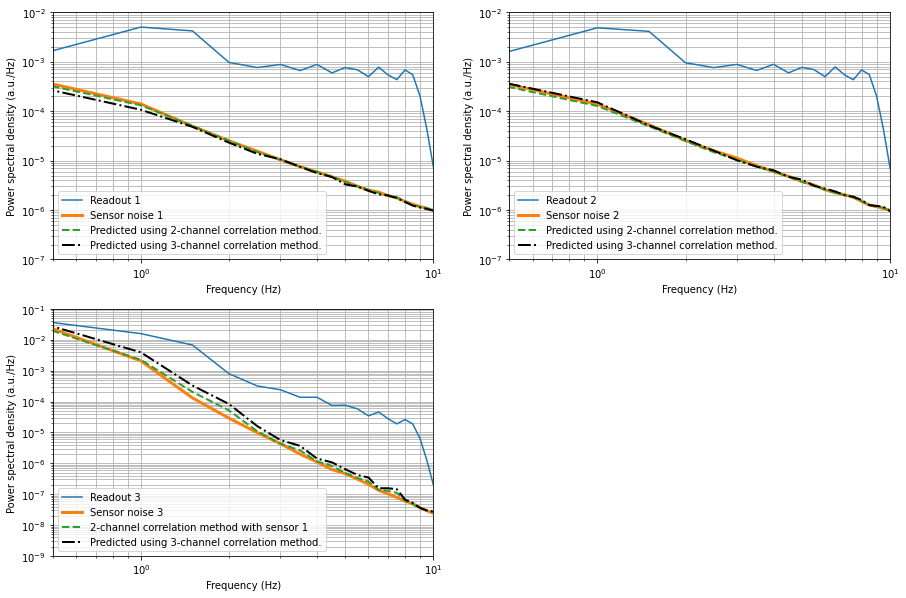
\includegraphics[width=1\linewidth]{figures/noise_estimation_using_correlation_methods}
	\caption{A comparison between the two-channel method and three-channel method.}
	\label{fig:noiseestimationusingcorrelationmethods}
\end{figure}
Fig.~\ref{fig:noiseestimationusingcorrelationmethods} shows a comparison between the two correlation methods from the notebook.
Sensor 1 and 2 has the same dynamics and noise PSDs, while sensor 3 has a completely different dynamics and noise PSD from the other two.
We used two-channel method to predict sensor noise 1 and 2, and used three-channel method for all of them.
We also used the two-channel method to predict sensor noise 3 using sensor 1 as a correlated sensor.
As shown in the figure, the predicted PSDs (shown in green dashed and dotted black lines) are very close to the actual sensor noises (shown in orange).
Here, we emphasize that using the two-channel method to predict self noise of sensor 3 is not a valid attempt as the other sensors don't have the same sensor dynamics and noise spectral density.
Hence, the green dashed line on the bottom left in Fig.~\ref{fig:noiseestimationusingcorrelationmethods} might be a fluke.
We used the same method to predict sensor noise 1 using sensor 3 as a correlated sensor and the prediction was clearly off (See the notebook for a figure).

\subsection{Frequency series fitting using mathematical optimization}
In this section, we will be discussing how to model frequency series using optimization methods.
In particular, we will discuss the fitting of noise spectum measurments in Sec.~\ref{sec:noise_modeling_baseline}, as a follow up of Sec.~\ref{sec:sensor_noise_measurement}.
And, the fitting of transfer function measurements is discussed in Sec.~\ref{sec:transfer_function_modeling}.
Some general tips on fitting frequency series using optimization is given in Sec.~\ref{sec:optimization_tips}.
In Sec.~\ref{sec:curve_fitting_examples}, we will exemplify the methods discussed.
We will be using mathematical optimization notations as given in appendix \ref{appendix:optimization}.
A good \verb|SciPy| reference on mathematical optimization can be found in \cite{scipy_mathematical_optimization}.
In this section, we will refer the word ``optimization'' to ``mathematical optimization'', which is to minimize an objective function/cost function.
\subsubsection{Noise spectrum modeling \label{sec:noise_modeling_baseline}}
In this section, we will discuss how to obtain a noise model from some sensor readout.
This can be useful if we need to have a analytic model or if we want to estimate the sensor noise from a signal sensor, whose readout is not purely noise-dominated.

If conditions in the Sec.~\ref{sec:displacement_sensors_baseline} and Sec.~\ref{sec:inertial_sensors_baseline}, such as fixing the suspensions or measuring the readout before installation, are not available, we cannot use the aforementioned noise measurement methods.
But, we can still estimate the sensor noise via a curve fitting procedure, if we have a noise model and if the signal sensor readout is not dominated at all frequencies, i.e. signal only dominates spectral partially.
An example of this situation would be a sensor that measures a damped sinusoidal, i.e.
\begin{equation}
	y(t) = x(t) + n(t) = C\Re{\left(e^{\sigma+i\omega_n t}\right)} + n(t)\,,
	\label{eqn:sensor_readout_damp_sinusoidal}
\end{equation}
where $x(t) = C\Re{\left(e^{\sigma+i\omega_n t}\right)}$ is the signal, $C$ is a real number, $\sigma$ is a negative real number, $\omega_n$ is the oscillation frequency, and $n(t)$ is the sensor noise.
In this case, the frequency spectrum of signal $x(t)$ is localized around $f=2\pi\omega_n$, while the frequency content of the sensor noise $n(t)$ spreads all frequencies, which is very typical for motion sensors in a suspension.

Say, we have measurements
\begin{equation}
	\hat{Y}(f) = \left[\hat{X}(f)^2 + \hat{N}(f)^2\right]^{\frac{1}{2}}\,,
	\label{eqn:sensor_measurement}
\end{equation}
where $\hat{Y}(f)$ is the ASD of the sensor readout $y(t)$, $\hat{X}(f)$ is the ASD of some signal $x(t)$, and $\hat{N}(f)$ is the ASD of the sensor noise $n(t)$ that we want to measure/model.
If we have a noise amplitude spectral model $\hat{N}_\mathrm{model}(f;\theta_{\hat{N}_\mathrm{model}})$, where $\theta_{\hat{N}_\mathrm{model}}$ is a list of parameters that defines the noise $\hat{N}_\mathrm{model}$, then we can do a curve fit to obtain the noise model.
A example choice of the noise model would be a quadrature sum
\begin{equation}
	\hat{N}_\mathrm{model}(f;\theta_{\hat{N}_\mathrm{model}})=\left[\left(\frac{N_a}{f^a}\right)^2 + \left(\frac{N_b}{f^b}\right)^2\right]^{\frac{1}{2}}\,,
	\label{eqn:noise_model}
\end{equation}
where $\theta_{\hat{N}_\mathrm{model}}=\{N_a,N_b,a,b\}$ are the model parameters.

The fit can be as simple as a least squares fit, i.e. by minimizing the sum of error squares cost function
\begin{equation}
	J_\mathrm{lsq}\mleft(\theta;A(m), B(m,\theta)\mright) = \sum_m^M\left[A(m)-B(m,\theta)\right]^2 w(m)^2\,,
	\label{eqn:least_squares_cost_function}
\end{equation}
where $\theta$ is some model parameters of an arbitrary analytical function $B(m,\theta)$, $A(m)$ is the measurement data, $m$ is a common parametrization of the series $A$ and $B$, and $w(m)$ is a user-designed weighting of each data point (weighting function).
Typical choices for $m$ could be time $t$, frequency $f$, or simply data index.
Minimization of Eqn.~\eqref{eqn:least_squares_cost_function} will give you the optimal parameters $\theta^*$ such that the best fit of data $A$ is the model $B(\theta^*)$.

We can use the least squares fit directly but this is not the best for fitting measurement data that is typically viewed in log or log-log plots, where the value of data points varies drastically in orders of magnitude.
Instead, we use $J_\mathrm{lsq}\mleft(\theta;\log{A(m)}, \log{B(m,\theta)}\mright)$.

As for the weighting function $w(f)$ (now as a function of frequency), an easy choice for our purpose would be
\begin{equation}
	w(f)=
	\begin{cases}
		0 &,\, f_\mathrm{lower}<f<f_\mathrm{upper} \\
		1 &,\, \textit{otherwise}
	\end{cases}
	\,,
	\label{eqn:weighting_function_frequency_bound}
\end{equation}
where $\left(f_\mathrm{lower},f_\mathrm{upper}\right)$ is a frequency bound that encloses frequency regions that has high SNR, indicated by the peak feature.
The choices of the design parameters $f_\mathrm{lower}$ and $f_\mathrm{upper}$ can't be easily told here as it requires users to look at the visualized data and make educated guesses.
Instead, we will demonstrate the choice of this bound in an example shown in Sec.~\ref{sec:curve_fitting_examples}.

To sum up, we have sensor data $\hat{Y}(f)$, which is an ASD (works for PSD as well.) as shown in Eqn.~\eqref{eqn:sensor_measurement}, and we would like to model the sensor noise $\hat{N}(f)$ with a model $\hat{N}(f;\theta_{\hat{N}_\mathrm{model}})$, where $\theta_{\hat{N}_\mathrm{model}}$ is a list of parameters of the sensor noise model.
We do so by minimizing the cost function
\begin{equation}
	\boxed{
		J_\mathrm{noise}\mleft(\theta_{\hat{N}_\mathrm{model}}\mright)=\sum_m^M\left[\log\hat{Y}(f_m)-\log\hat{N}_\mathrm{model}(f_m, \theta_{\hat{N}_\mathrm{model}})\right]^2 w(f)^2
	}\,,
	\label{eqn:noise_cost_function}
\end{equation}
where the weighting function $w(f)$ is given in Eqn.~\eqref{eqn:weighting_function_frequency_bound} and $f_m$ are the frequencies where the measured PSD and the model are evaluated.
The reason for using the log error $\log\hat{Y}(f) - \log\hat{N}_\mathrm{model}(f;\theta_{\hat{N}_\mathrm{model}})$ instead of the typical error is given in Sec.~\ref{sec:optimization_tips}, and will be obvious in the example section \ref{sec:curve_fitting_examples}.
Minimization gives best-fit parameters
\begin{equation}
	\theta_{\hat{N}_\mathrm{model}}^*=\arg\min{\theta_{\hat{N}_\mathrm{model}}} \hat{J}_\mathrm{noise}\mleft(\theta_{\hat{N}_\mathrm{model}}\mright)\,,
\end{equation} such that the noise model $\hat{N}_\mathrm{model}\mleft(f;\theta_{\hat{N}_\mathrm{model}}^*\mright)$ becomes a best fit of the noise spectral density $\hat{N}(f)$.
The minimization can be done using methods that will be discussed in Sec.~\ref{sec:optimization_tips}.
\subsubsection{Transfer function modeling \label{sec:transfer_function_modeling}}

\subsubsection{Some tips on using optimization \label{sec:optimization_tips}}
Minimization with measurement data can be done iteratively using optimization algorithms like gradient descent \cite{enwiki:1019572955} (local minimization) or stimulated annealing \cite{enwiki:1017509035} (global minimization).
We will not dive into the topic of mathematical optimization since it's a topic on it's own and is out of the scope of this document.
Instead, we will simply be using packages that are readily available.
A very useful Python submodule is \verb|scipy.optimize| \cite{scipy_optimize}.
It provides functions for both local minimization (\verb|scipy.optimize.minimize()|) and global minimization.
It comes with many popular algorithms such as the Nelder-Mead algorithm (\verb|scipy.optimize.minimize(..., method="Nelder-Mead")|) \cite{wiki:nelder_mead}, which is known to be good for optimization with noisy experiment data, or differential evolution \linebreak(\verb|scipy.optimize.differential_evolution()|) \cite{wiki:differential_evolution}.
The choice of algorithm is very subtle as different algorithms practically perform equally well for our purpose.
If you really need to know which one to use, try consulting \cite{scipy_mathematical_optimization}.
However, we do distinguish the choice between a local minimization algorithm and a global one.
The former can only be used when with guessed initial parameters, while the latter one can only be used when the boundaries of the parameters is known.
Typically, we\footnote{I mean I (Terrence)} prefer global optimization approaches because typically we don't know the parameters.
While the optimization result can depend on the initial guesses, having a poor guess would yield suboptimal results.

An important note on numerical optimization is parameter scaling \cite{wiki:preconditioner}.
We won't go into details.
The idea is to scale the parameters in such that they are all in the same scale, hence the cost function is equally sensitive to all parameters.
For some parameters $\theta=\{\theta_1,\theta_2\}$ that has a large dynamic range, it might be helpful if we optimize $\tilde{\theta}=\{\log\theta_1, \log\theta_2\}$ instead.
An example where this kind of rescaling is necessary is transfer function fitting with polynomial models, which have coefficients the vary in orders of magnitude.
Another example would be $N_a$ and $N_b$ from Eqn.~\eqref{eqn:noise_model}, which are noise levels that can also vary drastically.

Another useful pre-processing procedure would be to resample the data using an log-spaced frequency axis, instead of using the linearly spaced one as obtained during Fourier transform.
With linear-space frequency points, the majority of the data clusters at higher frequencies as viewed from a log-frequency axis, which create bias towards high frequency data.
As a result, the best-fit model might fit measurement data at higher frequencies better than that at lower frequencies.
A simple resample of the data will redistribute the data uniformly across the log-frequency axis.

\subsubsection{Examples \label{sec:curve_fitting_examples}}
\paragraph{Noise spectrum modeling}
Here, we will demonstrate how to use optimization to minimize cost functions \eqref{eqn:least_squares_cost_function} and \eqref{eqn:noise_cost_function} to model a sensor noise ASD $\hat{N}(f)$.
The notebook is available \href{https://kontrol.readthedocs.io/en/latest/tutorials/noise_spectrum_modeling_with_optimization.html}{here}.
We will assume a sensor readout $y(t)$ that follows Eqn.~\eqref{eqn:sensor_readout_damp_sinusoidal}, with a noise $n(t)$ that follows Eqn.~\eqref{eqn:noise_model}.
We will add measurement noise uniformly drawn from $[-3, 3]\,\mathrm{dB}$ to the sensor readout $y(t)$.

Fig.~\ref{fig:tutorialsnoisespectrummodelingwithoptimization10} shows the time series of the signal $x(t)$ and the frequency series $\hat{Y}(f)$, $\hat{N}(f)$, $\hat{X}(f)$, and the weighting function $w(f)$.
Here, the signal is
\begin{equation}
	x(t) = A\Re{\left(e^{\sigma+i\omega_n t}\right)},
\end{equation}
and we set $A=1$, $\sigma=-0.001$, $\omega_n=2\pi$.
The noise spectral density is
\begin{equation}
	\hat{N}(f) = \left[\left(\frac{N_{3.5}}{f^{3.5}}\right)^2+\left(\frac{N_1}{f^1}\right)^2\right]^\frac{1}{2}\,,
\end{equation}
where $N_{3.5}=\left(5\times10^{-7}\right)^\frac{1}{2}$ and $N_1=\left(1\times10^{-7}\right)^\frac{1}{2}$.
This these frequency dependencies ($-3.5$ and $-1$) are chosen to mimic the behavior of the geophone noise.
This kind of sensor noise profiles has large amplitude variations at different frequencies so it can be used as a benchmark problem for noise modeling.
So, the ASD of the sensor readout, in $\mathrm{dB}$ is
\begin{equation}
	20\log\hat{Y}(f) = 20\log\left[\hat{X}(f)^2 + \hat{N}(f)^2\right]^\frac{1}{2} + U(-3, 3)\,,
\end{equation}
where $U(a,b)$ is a random series drawn from a uniform distribution between $a$ and $b$.

In reality, the only information we have is the sensor readout $\hat{Y}(f)$, as given by the green curve shown in Fig.~\ref{fig:tutorialsnoisespectrummodelingwithoptimization10}.
From the plot, we see a peek feature around $0.7 ~ 2\,\mathrm{Hz}$, which indicates the presence of the signal $x(t)$.
This is something that we do not wish to model.
Hence, we set the weighting function
\begin{equation}
	w(f)=
	\begin{cases}
		0 & ,\,0.7<f<2\,\mathrm{Hz}\\
		1 & , otherwise.
	\end{cases}
	\,,
\end{equation}
so it filters out the part of the readout that we don't wish to model.
\begin{figure}[!h]
	\centering
	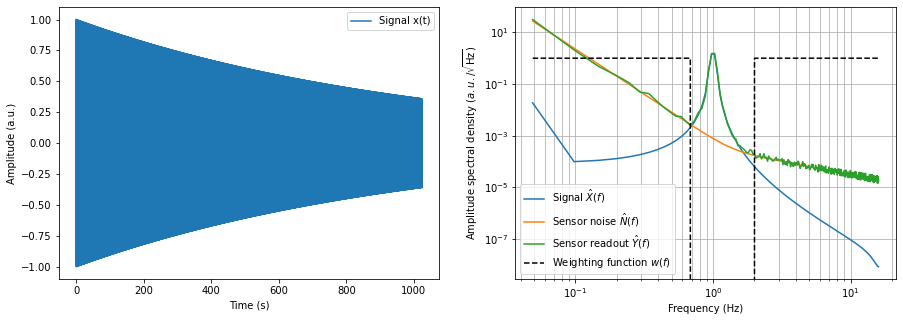
\includegraphics[width=1\linewidth]{figures/tutorials_noise_spectrum_modeling_with_optimization_1_0}
	\caption{(Left) Time series of the signal $x(t)$. (Right) Amplitude spectral densities of the readout $\hat{Y}(f)$, sensor noise $\hat{N}(f)$, signal $\hat{X}(f)$, and the designed weighting function $w(f)$.}
	\label{fig:tutorialsnoisespectrummodelingwithoptimization10}
\end{figure}

As for the model, we model ~\eqref{eqn:noise_model}.
We fit the measurement with 4 different configurations.
For the first two, we use least squares fit, which uses Eqn.~\eqref{eqn:least_squares_cost_function}, with model parameters $\theta_{\hat{N}_\mathrm{model}}=\{N_a, N_b, a, b\}$, and ``log parameters'' $\tilde{\theta}_{\hat{N}_\mathrm{model}}=\{\log N_a, \log N_b, a, b\}$, respectively.
For the other two, we use least squares fit with log error, which uses Eqn.~\eqref{eqn:noise_cost_function}, again with the two different sets of model parameters.
The motivation for using log parameters is discussed in Sec.~\ref{sec:optimization_tips}.


\begin{figure}[!h]
	\centering
	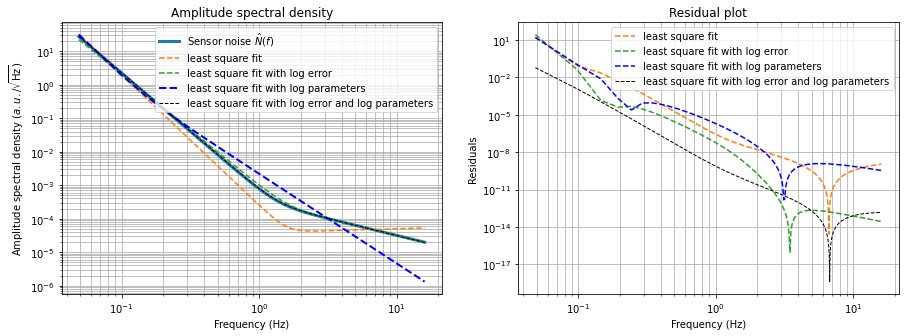
\includegraphics[width=1\linewidth]{figures/tutorials_noise_spectrum_modeling_with_optimization_8_0}
	\caption{(Left) Fitting results. (Right) Residuals, i.e. error squared.}
	\label{fig:tutorialsnoisespectrummodelingwithoptimization80}
\end{figure}

Fig.~\ref{fig:tutorialsnoisespectrummodelingwithoptimization80} shows the optimization results with the four configurations.
As can be seen on the left plot, least squares fit with log error yields noise models that fit the actual noise well across all frequencies.
But, the traditional least square fit fails at fitting the data at higher frequencies, where the amplitudes of the noise is orders of magnitude lower than that at lower frequencies.
Right plot in Fig.~\ref{fig:tutorialsnoisespectrummodelingwithoptimization80} shows the residuals, defined by the square error between the actual noise and the fit, of these four configuration.
As shown in the plot, modeling the noise with least square fit with log error and log parameters yields the best result in default settings.
This shows the importance in correct scaling of the model parameters.

For all these results, we used \verb|scipy.optimize.minimize()|, with default settings, to minimize the cost functions, and we start from an initial guess of $\{0, 0, 0, 0\}$ in all cases.
We emphasize that all these four configuration may perform equally well if we further tweak the optimization parameters in \verb|scipy.optimize.minimize()|, or using different optimization algorithms.
There are many optimization tweaks that can improve the fitting performance, but we won't discuss here.
The results shown in Fig.~\ref{fig:tutorialsnoisespectrummodelingwithoptimization80} only serves as a demonstration of how a careful design of the model and the cost functions can yield better results under the same settings.

\subsection{Control matrices}
In this section, we will discuss how control matrices (sensor matrices and actuation matrices) can be derived, and how to fine tune them (diagonalization).

As is discussed in Sec.~\ref{sec:suspension_commissioning_tasks_further_elaboration}, there are many sensors and actuators in a single stage of suspension.
And in fact, sensors and actuators mostly come in pairs for KAGRA suspensions.
For instance, at the preisolator stage, there are 3 linear variable differential transformers (LVDTs) (not counting inertial sensors), and 3 coil-magnetic actuators placed at close proximity to the LVDTs.
Another example would be the intermediate-mass stage, which has 6 optical sensors and electromagnetic actuator (OSEMs) or photo-reflective displacement sensors (PS).
One exception would be the optics stage which has four coil-magnetic actuators, while only have an optical lever that can measure displacements from 3 degrees of freedom (DoFs).
In principle, the number of independent sensors, or I should say, readouts, decides the number of degrees of freedom that we can measure.
The minimum number of sensors that is needed is at least the number of degrees of freedom that we want to measure.
And, so this is equivalent to saying that, the maximum number of degrees of freedom that we can measure, is the maximum number of sensors.
The same goes to actuators.

Having sufficient number of sensors and actuators at a stage gives us the possibility to sense or actuate the motion at different DoFs of a stage.
But, the sensors and actuators may not be aligned directly to the degrees of freedom that we would like to measure.
For example, the LVDTs at the preisolator stage are located at the outer edge of the preisolator table, which is circular in shape so three LVDTs are sensing the tangential displacement of the preisolator table at three different angles (see \cite{all_of_the_vibration} for a simple figure).
Therefore, the readouts must be transformed from the sensor basis to the basis that we would like to perform control.
The same goes to actuation.
This is done via control matrices.

The desired basis is typically Cartesian (longitudinal, transverse, and vertical) with Euler angles (roll, pitch, yaw).
The Cartesian basis is defined locally for each suspension, where longitudinal direction is typically the normal of the high-reflectivity (HR) side of the optics, vertical is up, and transverse is the direction such that the cross product of the longitudinal direction and transverse direction is vertical.
As for the angles, roll, pitch, and yaw are defined as the angular displacements along the longitudinal, transverse, and vertical axis, respectively.
These DoFs can be locally defined for each stages as well.
For example, we would say IP yaw, IM yaw, and TM yaw, which are yaw at the preisolator, intermediate mass, and optics, respectively.
But, in this section we will focus on stage-wise control matrices, i.e. not mixing sensor readouts from different stages.

In a nutshell, here is how control matrices are derived for each stage.
We express each sensor readout $y_i(t)$ as a superposition of the stage's displacements $x_j(t)$,
\begin{equation}
	y_i(t) = \sum_j^m C_{ij} x_j(t)\,,
\end{equation}
where $i=1,2,3,\dots,n$ where $n$ is the number of sensors, and $j=1,2,3,\dots,m$ where $m$ is the number of degrees of freedom, $C_{ij}$ is the matrix elements of a matrix $\mathbf{C}$ and $\mathbf{C}\in \mathbb{R}^{n\times m}$.
$C_{ij}$ is the coupling coefficient of displacements $x_j(t)$ to sensor  $y_i(t)$
Then, the sensing matrix, defined by a conversion that maps the sensor readouts to the stage displacements, is simply
\begin{equation}
	\mathbf{C}_{\mathrm{sensing}} = \mathbf{C}^{\dagger}\,,
\end{equation}
where $\mathbf{C}_\mathrm{sensing} \in \mathbb{R}^{m\times n}$, such that $\mathbf{x}(t) = \mathbf{C}_\mathrm{sensing}\mathbf{y}(t)$.

The same goes to actuation.
Suppose we have actuation signals $u_i(t)$ injected to the $i^\mathrm{th}$ actuator.
Since the actuators are not purely acting on a single DoF, the actuation signal reads (at DC only, at higher frequencies there's phase shift. To be discussed in Sec.~\ref{sec:control_matrices_frequency_dependent_matrices}),
\begin{equation}
	u_i(t) = \sum_j^m D_{ij} x_j(t)\,,
\end{equation}
where $i=1,2,3,\dots,n$ where $n$ is the number of actuators, $j=1,2,3,\dots,m$ where $m$ is the number of DoFs, and $D_{ij}$ is the matrix elements of a matrix $\mathbf{D}$ and $\mathbf{D}\in \mathbb{R}^{n\times m}$.
Here, different from $C_{ij}$, the scale of $D_{ij}$ doesn't not matter, so long as the row vectors $D_{ij}$ has a direction parallel to the actuation.
Again, the actuation matrix, defined by the matrix mapping the actuation to the stage displacements, is simply
\begin{equation}
	\mathbf{D}_\mathrm{actuation} = \mathbf{D}^{\dagger}\,,
\end{equation}
and $\mathbf{D}_\mathrm{actuation}\in\mathbb{R}^{m\times n}$, such that $\mathbf{x}(t) = \mathbf{D}_\mathrm{actuation}\mathbf{u}(t)$.

Now, initial control matrices can be determined from the location and orientation, i.e. from geometry, of the sensors and actuators with respect to the stage.
\cite{sr_suspension_diagonalization} and \cite{bs_suspension_diagonalization} gives detailed calculation of the actuation and sensing matrices for the SR suspensions and BS suspensions for all stages, except sensing for the optics stage.
The sensing of the optics stage utilizes an optical lever setup and the derivation is more involved.
The derivation of the initial sensing matrix of optical levers is given in \cite{sensing_matrices_oplev}.
Details of these initial control matrices will be be discussed here.

Having the initial matrices may not be sufficient as residual cross-couplings may still remain.
In Sec.~\ref{sec:control_matrices_sensing_matrices}, we will discuss how to modify the sensing matrices so each sensor readout measures one pure DoF.
In Sec.~\ref{sec:control_matrices_actuation_matrices}, we will discuss how to modify the actuation matrices so each actuation signal purely moves the stage in one direction (at one paricular frequency only).
In Sec.~\ref{sec:control_matrices_frequency_dependent_matrices}, we will discuss a more general actuation matrix, which is a transfer function matrix, i.e. frequency dependency.
These methods are referred to sensor and actuation ``diagonalization'' in KAGRA.


\subsubsection{Sensing matrices \label{sec:control_matrices_sensing_matrices}}
Sensor and actuation diagonalization are two separate procedures but, as we shall we, sensor diagonalization must happen before actuation diagonalization, as it depends on the sensing readouts.
When sensor diagonalization is performed, the actuators should be re-diagonalized if it was done with a different sensing matrix.
Now, let's say we have raw sensing signals $\mathbf{y}(t)=y_i(t)$, where $i=1,2,3,\dots,n$, and $n$ is the number of sensors we have.
These signals are what the sensors measure.
They can be raw voltage, or calibrated in some sort of displacement units.
We have a initial sensing matrix $\mathbf{C}_\mathrm{sensing}^\mathrm{initial}$ that we derived from the geometric location and the orientation of the sensors.
Hence, we have some displacement readouts
\begin{equation}
	\mathbf{x}_\mathrm{readout}(t)=\mathbf{C}_\mathrm{sensing}^\mathrm{initial}\mathbf{y}(t)=\mathbf{C}_\mathrm{coupling}\mathbf{x}(t)\approxeq\mathbf{x}(t)\,,
\end{equation}
where $\mathbf{x}(t)$ is the displacements of the suspensions that we would like to measure and $\mathbf{C}_\mathrm{coupling}$ is a coupling matrix, with off-diagonal terms being the cross-coupling coefficients.

If the initial sensing matrix is perfect, then the coupling matrix $\mathbf{C}_\mathrm{coupling}$ will be the identity matrix $\mathbf{I}$ such that $\mathbf{x}_\mathrm{readout}(t)=\mathbf{x}(t)$.
But, in general, this is not the case.
If the off-diagonal elements in the coupling matrix are not zero, then the displacement readouts $\mathbf{x}_\mathrm{readout}(t)$ are cross-coupled, and the goal of diagonalization is to adjust the sensing matrix so individual readout is only coupling to one degree of freedom.
To decouple the readouts, we simply need to modify the sensing matrix such that
\begin{equation}
	\boxed{
		\mathbf{C}_\mathrm{sensing} = \left(\mathbf{C}_\mathrm{coupling}\right)^{-1} \mathbf{C}_\mathrm{sensing}^\mathrm{initial}
}\ .
	\label{eqn:sensing_matrix_diagonalization}
\end{equation}
Depending on the suspensions' real-time model architecture, this can be done by multiplying an addition matrix after the initial sensing matrix, or it can be done by simply modifying the existing matrix.

To measure the coupling matrix $\mathbf{C}_\mathrm{coupling}$, we have to rely on resonance features of the suspension.
Some resonant modes of the suspension only involve a single direction.
If these modes have distinguishable frequencies from other modes, then we can estimate the off-diagonal coupling coefficients ratios between the $i^\mathrm{th}$ readout and $j^\mathrm{th}$ readout,
\begin{equation}
	\boxed{
		C_{\mathrm{coupling}, ij}=
		\begin{cases}
			\left\lvert\frac{X_{\mathrm{readout}, i}(s)}{X_{\mathrm{readout}, j}(s)}\right\rvert_{f=f_j}\,, & \angle\frac{X_{\mathrm{readout}, i}(s)}{X_{\mathrm{readout}, j}(s)}\Big\vert_{f=f_j}\approx 0\,,\\
			-\left\lvert\frac{X_{\mathrm{readout}, i}(s)}{X_{\mathrm{readout}, j}(s)}\right\rvert_{f=f_j}\,, & \angle\frac{X_{\mathrm{readout}, i}(s)}{X_{\mathrm{readout}, j}(s)}\Big\rvert_{f=f_j}\approx \pm \pi\,,\\
		\end{cases}
	}
\end{equation}
where $f_j$ is the resonance frequency of the $x_j$ degree of freedom and $X_{\mathrm{readout},i}(s)$ is the Laplace transform of the $i^\mathrm{th}$ readout of $\mathbf{x}_\mathrm{readout}(t)$.
And note here we have explicitly specify the $s$ dependency to distinguish transfer functions and matrices.

Here, a few assumptions are made.
First of all, assume that the suspension stages are oscillating to the extent the peaks in the spectrum are high enough for us to measure coupling ratios, or to say that the coupling ratios are small.
So, the suspensions must be excite via external actuation, typically using the actuators.
There're two ways this can be done, 1) we can use the actuators to give a ``kick'' to the suspension, i.e. impulse input, so it freely swings in damped oscillation or 2) we can inject white noise actuation to excite the modes.
Mathematically, the resulting spectrum should be the same, as an impulse input is effectively white noise in the frequency domain.
But, the white noise actuation might be easier to implement, as the damped oscillation excited by the impulse may result in low SNR towards steady-state.
Secondly, we assume that the sensors are calibrated such that the diagonal terms of the coupling matrix are ones.
Thirdly, we assume that the coupling ratios measured are purely due to linear readout cross-coupling so, if there's cross-coupling, the ratio between the readouts at resonance frequencies must have a 0 relative or $\pm \pi$ phase.
If the ratios has a phase that is not close to 0 or $\pm \pi$ but the magnitude of the ratios are not small, this would mean that the results are not conclusive so we should not assign the ratio to the coupling matrix.
This could happen due to low SNR, mechanical coupling, or other reasons that are not yet clearly studied.
Unless the reason is known, we should not remove these spurious cross-couplings as it would be overcompensating.

\subsubsection{Actuation matrices \label{sec:control_matrices_actuation_matrices}}
The idea for actuation diagonalization is similar to that of sensor diagonalization but with some minor differences.

Let's say we have raw actuation signals $\mathbf{u}(t)$ and displacements $\mathbf{x}(t)$.
These raw actuation signals are voltage or ``counts'' applied to the actuators, and the $\mathbf{u}(t)$ frame is in the actuator frame, which is not aligned to the displacements $\mathbf{x}$.
We wish to have actuations signals $\mathbf{u}_\mathbf{x}(t)$ that are parallel to the displacements $\mathbf{x}(t)$.
So $\mathbf{u}_\mathbf{x}(t)$ is something like actuation signal in longitudinal, transverse, \dots, etc, and this is the variable that the control system manupulates.
Whereas, the raw actuation signal $\mathbf{u}(t)$ is like actuation in first actuator, second actuator, \dots, etc.
The actuation signals need to be converted back to the raw actuation signals via multiplying the actuation signals by the actuation matrix, i.e.
\begin{equation}
	\mathbf{u}(t)=\mathbf{D}_\mathrm{actuation}\mathbf{u}_\mathbf{x}(t)\,,
\end{equation}
where $\mathbf{D}_\mathrm{actuation}$ is the actuation matrix.

Now, let's say we have initial actuation matrix $\mathbf{D}_\mathrm{actuation} = \mathbf{D}_\mathrm{actuation}^\mathrm{initial}$.
If the actuation is not diagonalized, the displacement due to actuation signals reads
\begin{equation}
	\mathbf{x}(t) = \mathbf{D}_\mathrm{coupling}\mathbf{u}_\mathbf{x}(t) \,,
	\label{eqn:coupled_displacement_actuation}
\end{equation}
where $\mathrm{D}_\mathrm{coupling}$ is the coupling matrix due to actuation.
The diagonal elements of $\mathbf{D}_\mathrm{coupling}$ are the actuation efficiencies, i.e. the transfer function gain from actuation to displacement.
Here, it would be tempting to multiply the actuation signal by a matrix $\left(\mathbf{D}_\mathrm{coupling}\right)^{-1}$, such that
\begin{equation}
	\mathbf{x}(t)=\mathbf{D}_\mathrm{coupling}\left(\mathbf{D}_\mathrm{coupling}\right)^{-1} \mathbf{u}_\mathbf{x}(t)\,.
\end{equation}
This will diagonalization the actuation, but it is not the ideal approach.
This is because this will make the actuation efficiencies from $\mathbf{u}_\mathbf{x}(t)$ to $\mathbf{x}(t)$ identically ones.
This may cause problems practically as we might want to compare actuation efficiencies or actuation transfer functions from previous measurements.
So instead, it follows that if we multiple the actuation signals $\mathbf{u}_\mathbf{x}(t)$ by $\left(\mathbf{D}_\mathrm{coupling}\right)^{-1}\mathbf{D}_\mathrm{efficiency}$ before converting to the raw actuation signals via the initial actuation matrix  $\mathbf{D}_\mathrm{actuation}^\mathrm{initial}$, then the actuation-displacement relation becomes
\begin{equation}
	\mathbf{x}(t) = \mathbf{D}_\mathrm{coupling}\left[\left(\mathbf{D}_\mathrm{coupling}\right)^{-1}\mathbf{D}_\mathrm{efficiency}\right]\mathbf{u}_\mathbf{x}(t)\,,
	\label{eqn:actuation_displacement_relation_diagonalized}
\end{equation}
where $\mathbf{D}_\mathrm{efficiency}$ is a diagonal matrix with elements being the actuation efficiencies at which the coupling matrix was measured.
The actuation efficiency matrix $\mathbf{D}_\mathrm{efficiency}$ is a free parameter that we can set.
So, for initial setup of the suspensions, this can be any arbitrary desired values.
However, for diagonalization, it's better to maintain the static gain of the actuation transfer functions, i.e. maintaining the previous actuation efficiencies.
This is equivalent to saying that we should set the actuation efficiency matrix to the diagonal elements of the actuation coupling matrix $\mathbf{D}_\mathrm{coupling}$
\begin{equation}
	\mathbf{D}_\mathrm{efficiency} = \text{diag}\left(\mathbf{D}_\mathrm{coupling}\right)\,.
\end{equation}

Now, coming back to the actuation matrix $\mathbf{D}_\mathrm{actuation}$.
If we must modify the actuation matrix for diagonalization (alternatively we can have matrices in between actuation signals and the initial actuation matrix in the system), then Eqn.~\eqref{eqn:actuation_displacement_relation_diagonalized} is equivalent to saying that we should modify the actuation matrix from the initial actuation matrix $\mathbf{D}_\mathrm{actuation}^\mathrm{initial}$ to
\begin{equation}
	\boxed{
		\mathbf{D}_\mathrm{actuation} = \mathbf{D}_\mathrm{actuation}^\mathrm{initial} \left(\mathbf{D}_\mathrm{coupling}\right)^{-1} \mathbf{D}_\mathrm{efficiency}
	}\ .
	\label{eqn:actuation_matrix_diagonalized}
\end{equation}

To measure the actuation coupling, we need to measure the displacement $\mathbf{x}(t)$ due to actuation $\mathbf{u}_\mathbf{x}(t)$.
However, to measure $\mathbf{x}(t)$, we can only rely on the sensing readout $\mathbf{x}_\mathrm{readout}(t)$ from Sec.~\ref{sec:control_matrices_sensing_matrices}.
Therefore, it is important to complete sensor diagonalization before actuation diagnalization such that $\mathbf{x}_\mathrm{readout}(t)=\mathbf{x}(t)$
Also, note that the level of diagonalization that actuation can achieve is at best the level of diagonalization of the sensors.
To measure the actuation coupling matrix, we need to inject actuation signals, typically in the form of a DC offset or a sinusoidal single-frequency line injection.
DC offset inject is good because it would mean that there's no relative-phase between actuation and displacement.
If we choose to use a line injection, we must choose frequency at which both diagonal transfer functions and cross-transfer functions has $0$ or $\pm\pi$ phase.
This is tricky because we can't measure the transfer function unless we diagonalize the actuation!
Another way to approach this is to choose a frequency $f_\mathrm{inject}$ such that the measured $\frac{\mathbf{X}(s)}{\mathbf{U}_\mathbf{x}(s)}\big\rvert_{f=f_\mathrm{inject}}$ has $0$ or $\pm\pi$ phase.
So, the actuation coupling matrix can be measured as
\begin{equation}
	\boxed{
		D_{\mathrm{coupling}, ij} =
		\begin{cases}
			\left\lvert\frac{X_{i}(s)}{U_{\mathbf{x}, j}(s)}\right\rvert_{f=f_\mathrm{inject}}\,, & \angle\frac{X_{j}(s)}{U_{\mathbf{x}, j}(s)}\Big\rvert_{f=f_\mathrm{inject}} \approx \angle\frac{X_{i}(s)}{U_{\mathbf{x}, i}(s)}\Big\rvert_{f=f_\mathrm{inject}}\,,\\
			-\left\lvert\frac{X_{i}(s)}{U_{\mathbf{x}, j}(s)}\right\rvert_{f=f_\mathrm{inject}}\,, & \angle\frac{X_{j}(s)}{U_{\mathbf{x}, j}(s)}\Big\rvert_{f=f_\mathrm{inject}} \approx \angle -\frac{X_{i}(s)}{U_{\mathbf{x}, i}(s)}\Big\rvert_{f=f_\mathrm{inject}}\,,
		\end{cases}	
}
\end{equation}
where $i,j = 1,2,3,\dots,n$ and $n$ is the degrees of freedom.

Here, there's a few caveats.
First of all, what we are doing here is \textbf{not} actually actuation diagonalization, instead, what we are trying to do is to align the actuators to the suspension stage's degrees of freedom.
But, this alignment has frequency dependency, if the cross-transfer functions are not zero, which is generally true.
This means what we cannot minimize actuation cross-coupling at all frequencies, except at a signal frequency, which is actually not that useful.
The good thing is that actuation diagonalization is not that important for local damping control, if controls are all engaged for all DoFs.
Actuation cross-coupling will be treated as disturbance from one DoF to another, and will be suppressed by active control.
However, actuation coupling will become important when suspension control is not engaged, such as during interferometer locking or observation.
Therefore, we need some way to actually diagnalize the actuations and this will be discussed in Sec.~\ref{sec:control_matrices_frequency_dependent_matrices}.

\subsubsection{Frequency dependent matrices \label{sec:control_matrices_frequency_dependent_matrices}}
As is discussed in Sec.~\ref{sec:control_matrices_actuation_matrices}, a scalar-valued actuation matrix is not useful for diagonalizing the actuators.
With a scalar actuation matrix, the actuation can only be diagonalized at a single frequency so actuation signals in one DoF at other frequencies can still other DoFs.
To correctly model the actuation system, we have to consider transfer function matrix, with input $\mathbf{U}_\mathbf{x}(s)=\left[U_{x_1}(s), U_{x_2}(s),\dots,U_{x_n}(s)\right]^T$ and output (displacement) $\mathbf{X}(s)=[X_1(s), X_2(s),\dots, X_n(s)]^T$, where $n$ is the number of  DoFs.
The input-output relation can be written as
\begin{equation}
	\mathbf{X}(s) = \mathbf{P}(s)\mathbf{U}_\mathbf{x}(s)\,,
\end{equation}
where the actuation plant $\mathbf{P}(s)$, i.e. the transfer function matrix is
\begin{equation}
	\mathbf{P}(s)=
	\begin{bmatrix}
		P_{11}(s) & P_{12}(s) & \dots & P_{1n}(s)\\
		P_{21}(s) & P_{22}(s) & \dots & P_{2n}(s)\\
		\dots & \dots & \ddots & \vdots\\
		P_{n1}(s) & P_{n2}(s) & \dots & P_{nn}(s)
	\end{bmatrix}\,,
\end{equation}
where $P_{ij}(s)$ is the SISO transfer function from the $j^\mathrm{th}$ actuation $U_j(s)$ to $i^\mathrm{th}$ displacement $X_i(s)$, and note that $P$/$\mathbf{P}$ here means plant/path/transfer function, and \textbf{not} power spectral density.
$\mathbf{P}(s)$ is the plant of the suspension and cannot be changed. 
The idea of diagonalization is to multiply the actuation signals by a transfer function matrix, i.e. ``the'' actuation matrix, such that the resultant off-diagonal transfer functions (cross-transfer functions) are zero.
Mathematically, we want to design an actuation matrix $\mathbf{D}_\mathrm{actuation}(s)$, such that
\begin{equation}
	\mathbf{X}(s) = \mathbf{P}(s)\mathbf{D}_\mathrm{actuation}(s)\mathbf{U}_\mathbf{x}(s)\,,
\end{equation}
and $\mathbf{P}(s)\mathbf{D}_\mathrm{actuation}(s)$ is a diagonal transfer function matrix, preferably with diagonal entries $P_{ii}(s)$.
It follows that if we set
\begin{equation}
	\mathbf{D}_\mathrm{actuation}(s) = \mathbf{P}(s)^{-1}\text{diag}\left(\mathbf{P}(s)\right)\,,
	\label{eqn:frequency_dependent_actuation_matrix}
\end{equation}
then we can obtain
\begin{equation}
	\begin{bmatrix}
		X_1(s)\\
		X_2(s)\\
		\vdots\\
		X_n(s)
	\end{bmatrix}
	=
	\begin{bmatrix}
		P_{11}(s) &  &  & \\
		& P_{22}(s) &  & \\
		&&\ddots&\\
		&&&P_{nn}(s)
	\end{bmatrix}
	\begin{bmatrix}
		U_{x_1}(s)\\
		U_{x_2}(s)\\
		\vdots\\
		U_{x_n}(s)
	\end{bmatrix}
	\,,
\end{equation}
which is exactly what we want, a diagonalized actuation plant.

There are at least ways to obtain the actuation matrix using Eqn.~\eqref{eqn:frequency_dependent_actuation_matrix}.
The first way is to measure the transfer functions $P_{ij}(s)$ as a complex-valued frequency series and then use a transfer function model to fit it using methods discussed in Sec.~\ref{sec:transfer_function_modeling}.
With the analytical form of the transfer functions, we can construct the transfer function matrix by evaluating Eqn.~\eqref{eqn:frequency_dependent_actuation_matrix}.
The calculation of the inverse of a transfer function matrix is rather involved as it's not easy to obtain the analytical form of the inverse.
If the matrix is small, we can easily express individual elements of the inverse transfer function matrix as a combination of the elements of the transfer function matrix.
However, this can become tedious as the number of DoFs exceed 3.
Alternatively, we can use the \verb|inv()| function in MATLAB, which apparently works with transfer function matrix \cite{invert_models_matlab}.
But, not every one can access MATLAB and we like open-source softwares like Python.
So, this brings us to the second way of obtaining the actuation matrix.
Instead of modeling the individual transfer functions $P_{ij}(s)$, we take the frequency series of the transfer functions and then compute the inverse of the transfer function matrix at each frequency so we can obtain the actuation matrix as a complex-valued frequency series using Eqn.~\eqref{eqn:frequency_dependent_actuation_matrix}.
From here, we can use transfer functions models to fit the individual elements of $\mathbf{D}_\mathrm{actuation}(s)$ using methods from Sec.~\ref{sec:transfer_function_modeling}.

\subsubsection{Examples}
Pending
\paragraph{Sensor diagonalization}
\paragraph{Actuation diagonalization}
\paragraph{Frequency dependent diagonalization}

\subsection{Inter-calibration}
\subsection{Sensor fusion}
As is discussed in Sec.~\ref{sec:suspension_commissioning_tasks_further_elaboration}, sensing noise is a limit of the control performance of the suspensions, and it dictates the best possible performance that we can obtain.
Therefore, it's very important to minimize the sensor noise as much as possible and as early as possible since controller design depends on the sensing noise.
One method that is used in KAGRA for minimizing sensor noise is sensor fusion.
Sensor fusion is a technique that combines multiple sensors into a virtual ``super sensor'' that has better performance compared to that of the individual sensors.
The sensors are measuring the a common signal but has different noise characteristics.

In KAGRA, sensor fusion is used mostly for the preisolator, where active seismic isolation is critical.
In particular, LVDTs and Geophones are blended using complementary filters so the displacement readouts at the preisolator benefits from the advantages from the goephones (seismic noise-free and low sensor noise at higher frequencies) and LVDTs (low sensor noise at lower frequencies).
Sensor correction is used to remove the seismic noise coupling from the LVDT readouts at the preisolator using the seismometer readout.
Strictly speaking, sensor correction also utilizes complementary filter.
For optimal performance, sensor correction should be considered as a complementary filter problem.
But, sensor correction was not conventionally considered this way during the first attempt in KAGRA \cite{sensor_correction_gain_tuning, comment_to_sensor_correction_gain_tuning}.
Instead, sensor correction filters were constructed as a high-pass filter using heuristics.
So, we will make a distinction between complementary filter problems and sensor correction filters in this section.
Also, note that, before sensor any sensor fusion tasks, the sensors involved must be inter-calibrated so to avoid weird calibration mismatch.
The inter-calibration techniques are given in Sec.~\ref{sec:inter-calibration}.

This section is organized as follows.
In Sec.~\ref{sec:complementary_filter}, we will discuss some predefined complementary filters and how to design and optimize the filter parameters.
In Sec.~\ref{sec:sensor_correction}, we will introduce the purpose of sensor correction and we will discuss how was it design and how can we improve it.
In Sec.~\ref{sec:sensor_fusion_examples}, we will provide examples on these complementary and sensor correction filters design.

\subsubsection{Sensor fusion using complementary filter \label{sec:complementary_filter}}
Fig.~\ref{fig:complementary_filter} shows the block diagram of a sensor fusion configuration using two filters $H_1(s)$ and $H_2(s)$ to blend two sensors that has different noise characteristics $N_1(s)$ and $N_2(s)$. 
\begin{figure}[!h]
	\centering
	
\includegraphics[width=64mm]{figures/complementary_filter}
	\caption{2-sensor blending using complementary filters}
	\label{fig:complementary_filter}
\end{figure}
As shown in the figure, the resultant ``super sensor'' readout has a super sensor noise $N_\mathrm{super}(s)$, and it's given by
\begin{equation}
	N_\mathrm{super}(s) = H_1(s)N_1(s) + H_2(s)N_2(s)\,.
\end{equation}
Note that we omitted the common signal that the sensors are measuring and simply focus on the noises.
Since we expect the super sensor readout to contain the original common signal, the  filters $H_1(s)$ and $H_2(s)$ must be complementary, as in
\begin{equation}
	H_1(s) + H_2(s) = 1\,.
\end{equation}
Alternatively, we can express the second filter $H_2(s)$ as $1-H_1(s)$, and so the super sensor noise is a function of one filter,
\begin{equation}
	N_\mathrm{super}(s; H_1(s)) = H_1(s)N_1(s) + \left[1-H_1(s)\right]N_2(s)\,.
\end{equation}
The amplitude spectral density of the super sensor noise is then
\begin{equation}
	\hat{N}_\mathrm{super}(f; H_1(s)) = \left[\left\lvert H_1(s) \right\rvert^2\hat{N}_1^2(f) + \left\lvert 1-H_1(s) \right\rvert^2\hat{N}_2^2(f)\right]^\frac{1}{2}\,,
\end{equation}
where $\hat{N}(s)$ denotes the amplitude spectral densities.
And here, clearly the goal is the design $H_1(s)$ such that some function $J$ of $\hat{N}_\mathrm{super}(f)$ is minimized.
The problem is stated as follow
\begin{equation}
	\minimize_{H_1(s)\in\mathcal{S}} J\mleft(\hat{N}_\mathrm{super}\mleft(f; H_1(s)\mright)\mright)\,,
	\label{eqn:cost_function_complementary_filter}
\end{equation}
where $J$ is some cost function and $\mathcal{S}$ is the set of proper transfer functions.
We didn't specify the cost function $J$ because this is a user-defined objective.
One of the typical choices of $J$ would be the (weighted) 2-norm \cite{norms_for_signals_and_systems}, which is equivalent to expected RMS of the weighted super sensor noise, i.e.
\begin{equation}
	J_2\mleft(H_1(s)\mright) = \left[\int_{-\infty}^\infty \, \hat{N}_\mathrm{super}\mleft(f;H_1(s)\mright)^2 w(f)^2\, df\right]^\frac{1}{2}\,,
	\label{eqn:cost_function_super_sensor_noise_rms}
\end{equation}
where, again, $w(f)$ is some specified weighting function according to specific requirements of the sensor.
Another typical choice of $J$ would be the (weighted) $\infty$-norm \cite{norms_for_signals_and_systems}, peak of the weighted spectral density of the super sensor noise, i.e.
\begin{equation}
	J_\infty\mleft(H_1(s)\mright) = \sup_{f} \left(\hat{N}_\mathrm{super}\mleft(f;H_1(s)\mright)w(f) \right) \,,
\end{equation}
where $\sup()$ denotes the supremum and $w(f)$ in this case would be the inverse of the frequency dependent specification of the sensor noise.
With all that said, these optimization problem defined by Eqn.~\eqref{eqn:cost_function_complementary_filter} may not be easy to solve, as parameterizing the transfer function space $\mathcal{S}$ is not easy.
Instead, these problems are solved using modern control methods like $\mathcal{H}_2/\mathcal{H}_\infty$ methods \cite{feedback_control_theory}, which is rather involved and will not be discussed here.
In a recent article, sensor correction filters (a type of complementary filter) used in LIGO \cite{low_frequency_vibration_isolation_hua} was reproduced using $\mathcal{H}_\infty$ synthesis using frequency dependent specifications by LIGO \cite{complementary_filters_shaping_using_h_infinity_synthesis}.
Unlike that in \cite{low_frequency_vibration_isolation_hua}, method in \cite{complementary_filters_shaping_using_h_infinity_synthesis} are extremely useful in optimizing IIR filters that is directly implementable to KAGRA's current digital system and therefore should be considered\footnote{This is part of my research actually.}.
However, we will only mention this here and details of these advanced methods will be discussed in the advance method section, i.e. Sec.~\ref{sec:suspension_commissioning_advanced_methods}.

Instead of fancy optimization approaches, we will discuss heuristic methods that were used to design complementary filters in KAGRA.
Here, we will present two methods used previously: 1) Predefined filters \cite{Sekiguchi:2016bmv, Heijningen:2018evm}, and 2) Filter shaping according to sensing noises \cite{low_frequency_optimization_and_performance_of_advanced_virgo_seismic_isolation_system}.
The two methods we discuss here will require a sensor noise measurement or modeling prior.
So be sure to check Sec.~\ref{sec:sensor_noise_measurement} and Sec.~\ref{sec:noise_modeling_baseline}.
Also be sure that those noise spectral densities are available before doing anything related to complementary filters.

Throughout the discussion, we will be referring noise $N_1$ to the seismic noise-coupled LVDT readout noise, see Sec.~\ref{sec:sensor_correction} for why this is the case, and $N_2$ to the geophone noise.
The ASD of the LVDT readout noise is defined as
\begin{equation}
	\hat{N}_1(f) = \left[ \hat{N}_\mathrm{LVDT}(f)^2 + \hat{N}_\mathrm{seismic}(f)^2 \right]^\frac{1}{2}\,,
\end{equation}
where $\hat{N}_\mathrm{LVDT}(f)$ is the ASD of the LVDT self-noise, which has a $f^{-0.5}$ dependency at low frequency and $f^{0}$ dependency at higher frequencies, and $\hat{N}_\mathrm{seismic}(f)$ is the ASD of the seismic noise.
The ASD of the geophone noise is simply
\begin{equation}
	\hat{N}_2(f) = \hat{N}_\mathrm{geophone}(f)\,,
\end{equation}
where $\hat{N}_\mathrm{geophone}$ is the geophone self-noise that has a $f^{-3.5}$ dependency at low frequency and $f^{-1}$ dependency at higher frequencies.
The amplitude spectral densities of these noises are plotted in Fig.~\ref{fig:sensornoisesforcomplementaryfilter}\footnote{I've altered the seismic noise at frequency $<0.4\,\mathrm{Hz}$ to omit the seismometer noise.}.
\begin{figure}[!h]
	\centering
	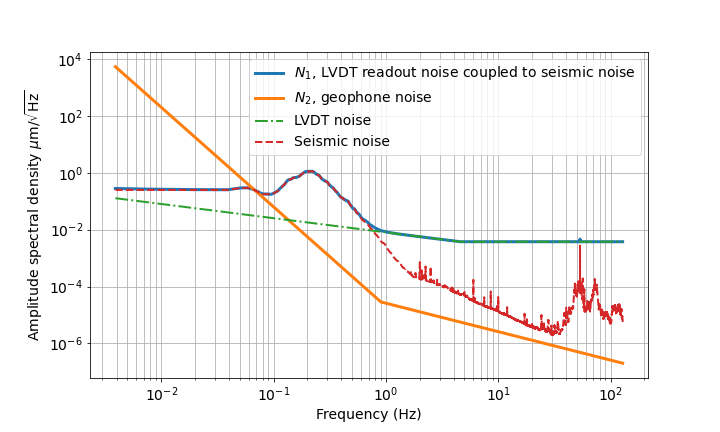
\includegraphics[width=0.7\linewidth]{figures/sensor_noises_for_complementary_filter}
	\caption{Amplitude spectral density of various noises. Blue: LVDT readout noise coupled to seismic noise. Orange: geophone noise. Green dash-dot: LVDT self-noise. Red dashed: Seismic noise from \cite{seismic_noise_kagra}. Note that the seismic noise was measured with seismometers so there're features at higher frequencies that are not really seismic noise, but are sensing artifacts. }
	\label{fig:sensornoisesforcomplementaryfilter}
\end{figure}

\paragraph{Predefined Filters}
In \cite{Sekiguchi:2016bmv} and \cite{Heijningen:2018evm}, sensor fusion using complementary filters to blend LVDTs and geophones at the preisolator stage was briefly discussed.
In \cite{Sekiguchi:2016bmv}, a predefined complementary filter was proposed,
\begin{equation}
	H_1(s;f_b) = \frac{35(2\pi f_b)^4 s^3 + 21(2\pi f_b)^5 s^2 + 7(2\pi f_b)^6 s + (2\pi f_b)^7}{(s+2\pi f_b)^7}\,,
	\label{eqn:complementary_filter_sekiguchi}
\end{equation}
where $f_b$ is the blending frequency at which $\lvert H_1(s)\rvert$ meets $\lvert H_2(s) \rvert$, and $H_2(s)=1-H_1(s)$.
Fig.~\ref{fig:sekiguchicomplementaryfilter} shows an example of Eqn.~\eqref{eqn:complementary_filter_sekiguchi} with blending frequency at $1\,\mathrm{Hz}$.
A simpler one was proposed in \cite{Heijningen:2018evm} but that was for Virgo so we won't mention it here.
\begin{figure}[!h]
	\centering
	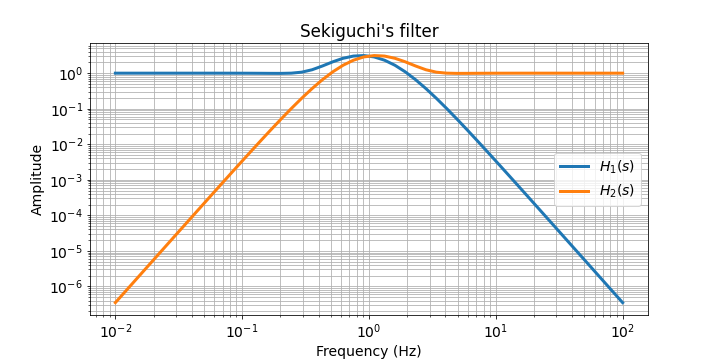
\includegraphics[width=0.7\linewidth]{figures/sekiguchi_complementary_filter}
	\caption{Example complementary filter Eqn.~\eqref{eqn:complementary_filter_sekiguchi} with $f_b=1\,\mathrm{Hz}$.}
	\label{fig:sekiguchicomplementaryfilter}
\end{figure}
The choice of filter shape defined in Eqn.~\eqref{eqn:complementary_filter_sekiguchi} is simple, i.e. the complementary filter $H_2(s)$ is a high-pass filter with fourth-order roll-off at lower frequencies.
The choice of this roll-off is designed to filter out the $f^{-3.5}$ geophone noise\footnote{In this sense, any forth-order high-pass filter should fulfill the purpose. The use of Eqn.~\eqref{eqn:complementary_filter_sekiguchi} is not really justified here. This is why I don't like the predefined filter approach.} as shown in Fig.~\ref{fig:sensornoisesforcomplementaryfilter}.
In \cite{Sekiguchi:2016bmv}, it was also mentioned the sensor noise would be minmized if the choice of blending frequency $f_b$ would be at the cross-over frequency of the two noises\footnote{The statement is vague. What does it mean by minimized? Minimized in what sense? In RMS? Or in peak amplitude?}, i.e. around $70\,\mathrm{mHz}$ in our case.

This method is indeed very simple to implement.
But, there are some caveats and problems to be noted.
First of all, we should note that this method is by definition suboptimal since the shape of the filter defined in Eqn.~\eqref{eqn:complementary_filter_sekiguchi} is hardly justified.
For example, what happens if we switched sensors, say, from geophones to accelerometers?
The noise profile would completely changed and so we might need a different roll-off for the accelerometer.
In this sense, having a predefined filter is not really general enough.
Also, we must note that there will be noise amplification around the blending frequency as shown in Fig.~\ref{fig:sekiguchicomplementaryfilter}.
So, in some extreme case, we might get worsened noise RMS/peak magnitude if the blending frequency is not placed properly.
Also, it's worth pointing out that the low-pass filter has a forth-order roll-off at high frequencies as well.
According to the design logic in \cite{Sekiguchi:2016bmv}, since the LVDT noise has a $f^{0}$ frequency dependency at higher frequencies, it's only required to have a first-order roll-off.
This would mean that the filter is a bit overkilled for the purpose of filtering LVDT noise.
So, why not design a complementary filter that composes of a first-order low-pass and a forth-order high-pass?
In this case, we might even get lower noise amplification at the blending frequency.
Nevertheless, what about the seismic noise coupling we see in the LVDT readout?
Shouldn't we design the complementary filter to account for the microseism around $200\,\mathrm{mHz}$?

\paragraph{Filter shaping according to sensing noises}
This brings us to the method used in \cite{low_frequency_optimization_and_performance_of_advanced_virgo_seismic_isolation_system}, filter shaping according to the sensor noise.
This method was brought to KAGRA by suspension experts in Virgo.
However, this method is closed-source and is not well known in KAGRA, even if those filters have been installed to the Type-A suspensions.
Therefore, here, I would like to reverse-engineer this approach.
I have used optimization methods to optimize complementary filters by minimizing various cost functions including the expected RMS of super sensor noise, i.e. Eqn.~\eqref{eqn:cost_function_super_sensor_noise_rms}, and the optimized filters strongly resembles those filters designed by this method.
So, personally, I think this is a slightly superior method compared to the predefined filter method in \cite{Sekiguchi:2016bmv, Heijningen:2018evm}.
To use this method, it's required to have good knowledge in filter shaping.
And so, this method can only be used by experts and it's likely to be irreproducible.
This is the downside of this method.

This method relies on designing a general filter/transfer function
\begin{equation}
	H_1(s;\theta_{H_1}) = \frac{\prod_i^{n_z}\left( s/z_i+1\right)}{\prod_j^{n_p} \left(s/p_j+1\right)}\frac{\prod_m^{n_{cz}} \left( \frac{1}{\omega_m^2}s^2 + \frac{1}{q_m \omega_m}s + 1 \right)}{\prod_n^{n_{cp}} \left(\frac{1}{\Omega_n^2}s^2 + \frac{1}{Q_n \Omega_n}s + 1 \right)}\,,
	\label{eqn:complementary_filter_general}
\end{equation}
where, $\theta_{H_1}$ are the design parameters $\left[z_i,p_j,\omega_m,q_m,\Omega_n,Q_n,n_z,n_p,n_{cz},n_{zp}\right]^T$, $z_i,p_j\in\mathbb{R}^+$ are the angular frequencies of the simple zeros and simple poles, $\omega_m,\Omega_n\in\mathbb{R}^+$ are the angular frequencies of the complex zeros and complex poles\footnote{Here, we defined complex zeros and poles as a second-order section in the numerator and the denominator respectively.}, $q_m,Q_n\in\mathbb{R}^+$ are the quality factors of the complex zeros and complex poles, and $n_z$, $n_p$, $n_{cz}$, and $n_{cp}$ are the number of zeros, poles, complex zeros, and complex poles, respectively.
Here, we have four types of elements, simple zeros $(s/z_i+1)$, simple poles $(\frac{1}{s/p_i+1})$, complex zeros $(\frac{1}{\omega_m}s^2+\frac{1}{q_m\omega_m}s+1)$, and complex poles $(\frac{1}{\frac{1}{\Omega_m}s^2+\frac{1}{Q_m\Omega_m}s+1})$, and the filter is defined as the produce of these elements.
The effect of these element in the magnitude response of the filter is well understood.
A simple zero will increase the slope of the magnitude response by 1 order per decade starting from the location of the zero $z_i$, while a simple pole will decrease the slope at the pole $p_j$ instead.
A complex zero will create a notch at the complex zero frequency $\omega_m$ and will increase the slope of the magnitude response by 2 orders per decade.
All these features combined can make any filter shape.
So unlike Eqn.~\eqref{eqn:complementary_filter_sekiguchi}, Eqn.~\eqref{eqn:complementary_filter_general} is maximally flexible.
This is also the reason why it can be hard to design.

\begin{figure}[!h]
	\centering
	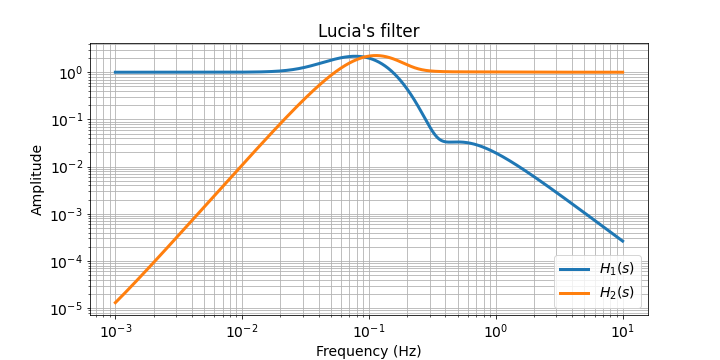
\includegraphics[width=0.7\linewidth]{figures/lucia_complementary_filter}
	\caption{Example complementary filter designed using method in \cite{low_frequency_optimization_and_performance_of_advanced_virgo_seismic_isolation_system}.}
	\label{fig:luciacomplementaryfilter}
\end{figure}
Fig.~\ref{fig:luciacomplementaryfilter} shows an example filter from \cite{low_frequency_optimization_and_performance_of_advanced_virgo_seismic_isolation_system}.
This filter may not be designed for KAGRA's sensors, but the concept is transferable.
Here, we will first qualitatively describe what is the rationale behind the design.
And then, we will do a break down of the transfer function expression of the filters in Fig.~\ref{fig:luciacomplementaryfilter} and attempt to reconstruct a filter like that.

The idea of this design goes as follows.
For the low-pass filter $H_1(s)$, we would like a $2^\mathrm{nd}$-order roll-off at high frequencies.
As for the high-pass $H_2(s)$, we are looking for a $3^\mathrm{rd}$-order roll-off at lower frequencies.
These roll-off orders are designed according to the noise amplitude spectral densities $\hat{N}_1(f)$ and $\hat{N}_2(f)$.
We can choose the roll-off order based on arguments in \cite{Sekiguchi:2016bmv}.
For example, if we expect the noise $\hat{N}_2(f)$ to have a $f^{-3.5}$ frequency dependency at lower frequencies, then the filter $H_2(s)$ should have at least that order of roll-off, i.e. $4^\mathrm{th}$-order roll-off.
Alternatively, the relative order between $\hat{N}_1(f)$ and $\hat{N}_2(f)$ is considered.
For example, if $\hat{N}_1(f)$ has a frequency dependency of $f^{-0.5}$ at lower frequencies and $\hat{N}_2(f)$ has a frequency dependency of $f^{-3.5}$ at lower frequency, the relative order is 3.
This means a $3^\mathrm{rd}$-order roll-off for $H_2(s)$ is sufficient so the noise $\hat{N}_2(f)$ not over-suppressed.
This is more optimal since over-suppressing would necessarily mean more noise-amplification around the blending frequency (See Bode's sensitivity integral for more details \cite{wiki:bode's_sensitivity_integral}.).
Like-wise, we can choose the roll-off for the low-pass following the same argument.
But in this case, $2^\mathrm{nd}$-order was chosen for whatever reason.
Another main difference between filters in Fig.~\ref{fig:luciacomplementaryfilter} and Fig.~\ref{fig:sekiguchicomplementaryfilter} is the ``notch'' in the low-pass filter at around $0.4\,\mathrm{Hz}$.
The low-pass filter is designed to have a higher-order roll-off around $0.1$ to $0.4\,\mathrm{Hz}$ for the purpose of filtering out the microseism around $0.2\,\mathrm{Hz}$.
The (secondary) microseism \cite{wiki:microseism} is a bump at around $0.2\,\mathrm{Hz}$ in the seismic noise spectrum, which is obviously visible in $N_1$ (blue curve) in Fig.~\ref{fig:sensornoisesforcomplementaryfilter}.
To prevent over-filtering, the low-pass returns to the $2^\mathrm{nd}$-order filtering at higher frequencies.
With these design features, the shapes of the low-pass and high-pass are roughly fixed except the blending frequency.
The blending frequency is the chosen to be high enough such that the inertial sensing noise at lower frequencies does not compromise the expected RMS of the super sensor noise.
Again, this will be around the cross-over frequency of the two sensing noises.

Now, let's reverse-engineer the filter shown in Fig.~\ref{fig:luciacomplementaryfilter} and see if we can design something similar.
The low-pass filter\footnote{I was given the filter by Lucia herself a few years ago.} shown in figure is expressed as
\begin{equation}
	H_1(s) = \frac{\left(\frac{1}{\omega_1^2}s^2+\frac{1}{q_1\omega_1}s+1\right)\left(\frac{1}{\omega_2^2}s^2+\frac{1}{q_2\omega_2}s+1\right)\left(\frac{1}{\omega_3^2}s^2+\frac{1}{q_3\omega_3}s+1\right)}{(s/p_1+1)^5(s/p_2+1)^3}\,,
	\label{eqn:complementary_low-pass_filter_lucia}
\end{equation}
where $\frac{p_1}{2\pi} = 0.12\,\mathrm{Hz}$, $\frac{p_2}{2\pi} = 0.25\,\mathrm{Hz}$, $\frac{\omega_1}{2\pi}=\frac{\omega_2}{2\pi} = 0.35\,\mathrm{Hz}$, $\frac{\omega_3}{2\pi} = 0.031272069\,\mathrm{Hz}$, $q_1 = 2$, $q_2 = 1.1$, and $q_3 = 0.64417749$.
From these values, we immediately see part of the story behind the design: the poles and the first two complex zeros are designed values while the third complex zero is passively derived numerically.
The reason why we cannot assign all parameters is because we want the complementary filter
$H_2(s)=1-H_1(s)$ to be a third-order high-pass filter.
This necessarily means that $H_2(s)$ must have 3 zeros at $0\,\mathrm{Hz}$ (or negligibly low frequency), i.e. $H_2(s) = \frac{s^3\dots}{\dots}$, and no poles between the blending frequency and $0\,\mathrm{Hz}$.
While $H_2(s) = 1-H_1(s) = \frac{\dots}{\left(s/p_1+1\right)^5\left(s/p_2+1\right)^3}$ that $H_1(s)$ and $H_2(s)$ to share the same poles, this guarantees that there will be no poles in $H_2(s)$ before the blending frequency, which will be slighly before $\frac{p_1}{2\pi}$.

Now, let's write $H_1(s)$ in a more general transfer function form
\begin{equation}
	H_1(s) = \frac{B(s)}{A(s)} = \frac{\sum_{i=0}^6 b_is^i}{\sum_{j=0}^8 a_js^j}\,,
	\label{eqn:complementary_low-pass_filter_lucia_polynomial}
\end{equation}
where $B(s)$ and $A(s)$ are the numerator and denominator polynomials of the $H_1(s)$ transfer function and $b_i$ and $a_j$ are the polynomial coefficients.
And, as for $H_2(s)$, it becomes
\begin{equation}
	H_2(s) = 1-H_1(s) = \frac{\sum_{j=0}^8 a_js^j - \sum_{i=0}^6 b_is^i}{\sum_{j=0}^8 a_j s^j}\,.
\end{equation}
So it follows that $a_2-b_2=a_1-b_1=a_0-b_0=0$ are the requirements, if we want $H_2(s) = \frac{s^3\dots}{\dots}$, i.e. a $3^\mathrm{rd}$-order high-pass filter.
Inspecting Eqn.~\eqref{eqn:complementary_low-pass_filter_lucia}, we see that $a_0=b_0=1$ so $a_0-b_0=0$ is automatically satisfied.
This means what we still need to engineer $b_2$ and $b_1$ so they equals to $a_2$ and $a_1$ respectively.
This explains why there are two passively derived values, $\omega_3$ and $q_3$, in Eqn.~\eqref{eqn:complementary_low-pass_filter_lucia}.
Let's assume that we designed other parameters (we shall explain this later) except $\omega_3$ and $q_3$.
Now, we just need to solve for them algebraically.
Plugging in $\frac{p_1}{2\pi} = 0.12\,\mathrm{Hz}$, $\frac{p_2}{2\pi} = 0.25\,\mathrm{Hz}$ into $A(s) = (s/p_1+1)^5(s/p_2+1)^3$, we get
\begin{equation}
	a_2=31.47148543 \quad\text{and}\quad a_1=8.54131528\,.
\end{equation}
Expanding $B(s)=\left(\frac{1}{\omega_1^2}s^2+\frac{1}{q_1\omega_1}s+1\right)\left(\frac{1}{\omega_2^2}s^2+\frac{1}{q_2\omega_2}s+1\right)\left(\frac{1}{\omega_3^2}s^2+\frac{1}{q_3\omega_3}s+1\right)$,
we get
\begin{equation}
	b_2 = \frac{1}{\omega_1^2} + \frac{1}{\omega_2^2} + \frac{1}{\omega_3^2} + \frac{1}{q_1\omega_1 q_2\omega_2} + \frac{1}{q_1\omega_1 q_3\omega_3} + \frac{1}{q_2\omega_2 q_3\omega_3}\,,
	\label{eqn:b_2_unsolved}
\end{equation}
and
\begin{equation}
	b_1 = \frac{1}{q_1\omega_1}+\frac{1}{q_2\omega_3}+\frac{1}{q_3\omega_3}\,.
\end{equation}
By equating $b_1=a_1=8.54131528$ and substituting $\frac{\omega_1}{2\pi}=\frac{\omega_2}{2\pi} = 0.35\,\mathrm{Hz}$, $q_1 = 2$, and $q_2 = 1.1$, we get
\begin{equation}
	\frac{1}{q_3\omega_3} = 7.9005615330066545\,.
	\label{eqn:1_over_q3_omega3}
\end{equation}
Substituting Eqn.~\eqref{eqn:1_over_q3_omega3} $\frac{\omega_1}{2\pi}=\frac{\omega_2}{2\pi} = 0.35\,\mathrm{Hz}$, $q_1 = 2$, $q_2 = 1.1$, and $b_2=a_2=31.47148543$ into \eqref{eqn:b_2_unsolved} and solve for $\omega_3$,
we get
\begin{equation}
	\begin{split}
		\frac{1}{\omega_3^2} &= 25.901625838545005\\
		\frac{\omega_3}{2\pi} &= 0.03127206923221885\,\mathrm{Hz}\,,
	\end{split} 
\end{equation}
where we of course reject the negative values corresponds to an unstable zero.
This matches the initial statement where we say $\frac{\omega_3}{2\pi} = 0.031272069\,\mathrm{Hz}$ is a derived value.
Solving for $q_3$, and not surprisingly, we get
\begin{equation}
	\begin{split}
		q_3 &= \frac{1}{7.900\dots\omega_3}\\
		&= 0.6441775018514415
	\end{split}
\end{equation}
which also equals the inital statement where we say $q_3 = 0.64417749$ is a derived value.

Now, let's see how are the other parameters decided.
First of all, let's remind ourselves what are the requirements of this filter.
The low-pass filter $H_1(s)$ has to have second-order roll-off at higher frequencies.
This means that the order of the denominator polynomial $A(s)$ has to at least 2.
We said that the high-pass filter $H_2(s)$ has to have third-order roll-off.
While $H_2(s) = 1-H_1(s) = \frac{A(s)-B(s)}{A(s)}$, and the order of $B(s)$ is less than that of $A(s)$, the order of $A(s)$ must be at least 3.
Now, as mentioned we need to have 2 derived parameters in $B(s)$ so the order of $B(s)$ is at least 2.
Since $H_1(s$ is designed to have second-order roll-off, the relative order between $B(s)$ and $A(s)$ must be 2, so now the order of $A(s)$ must be at least 4.
Now, this is the tricky part.
By inspecting the $N_1$ noise in Fig.~\ref{fig:sensornoisesforcomplementaryfilter}, we see that the microseism is roughly 2 orders of magnitude higher than that of the geophone noise $N_2$.
While the microseism noise spans around half a decade, to completely suppress it would require a $4^\mathrm{th}$-order roll-off before the microseism.
In other words, we would require 4 additional order in $A(s)$ to suppress this, and also 4 addition order in $B(s)$ to cancel the high-order roll-off so to retain a $2^\mathrm{nd}$ order roll-off at higher frequencies.
These constrain $A(s)$ to be an $>8^\mathrm{th}$-order polynomial and $B(s)$ to be an $>6^\mathrm{th}$-order polynomial.
This justifies the form as shown in Eqn.~\eqref{eqn:complementary_low-pass_filter_lucia_polynomial}.
Converting from Eqn.~\eqref{eqn:complementary_low-pass_filter_lucia_polynomial} to Eqn.~\eqref{eqn:complementary_low-pass_filter_lucia} is purely a designer's choice as it's free to construct the polynomials using either simple zeros/poles or complex zeros/poles.
However, it's important to set the frequencies of the zeros and poles according to the purpose.
Here, as we would like to filter out the microseism, $p_1$ was chosen to be at $0.12\,\mathrm{Hz}$ so the low-pass roll-offed before the microseism frequency.
The choice of the order $p_1$ is $5$ which would be arguable as it might the roll-off might be reduced to $3^\mathrm{rd}$-order if one of the frequencies of the complex zeros is lower than that of $p_1$, which is actually the case.
The frequency of $p_2$ is chosen to be $0.25\,\mathrm{Hz}$, which is not that important so long as it's
in between the frequencies of the two complex zeros, which is $0.35\,\mathrm{Hz}$.
The frequencies of the complex zeros are chosen to be slightly higher than that of the microseism so the low-pass filter returns to a the final designed $2^\mathrm{nd}$-order roll-off.
The Q factors for the first and second are tunable parameters so to finely adjust the blending frequency as well as the suppression needed at the complex zeros frequencies.
The ended up irrelevant as they were set to very low.
At last, as mentioned, the frequency and the Q factor of the final complex zero was passive determined by requiring the high-pass filter $H_2(s)$ to have $3^\mathrm{rd}$-order roll-off.
This is how a complementary filter is designed and justified.

Now, this will become very tedious but there's a resolution.
As mentioned before, if we use optimization approach to minimize the super sensor noise by optimize an arbitrary $H_1(s)$ that has a $6^\mathrm{th}$-order numerator and $8^\mathrm{th}$-order numberator, then the result will be very similar to that shown in Fig.~\ref{fig:luciacomplementaryfilter}.
And, it'll be arguably better.
But let's not overcrowd this section and left this discussion to a later section (Sec.~\ref{sec:suspension_commissioning_advanced_methods}).

\subsubsection{Sensor correction \label{sec:sensor_correction}}
\subsubsection{Examples \label{sec:sensor_fusion_examples}}

\subsection{Sensor correction \label{sec:sensor_correction}}
\subsection{Time series simulation of a given PSD}
\subsection{Controller design}

